\chapter{Methodology}
\clearpage

\section{Introduction}
Automated skin lesion classification enables early and accurate diagnosis of dermatological pathologies. In this study, we develop a robust end-to-end pipeline—from data acquisition and augmentation to model training, evaluation, and edge deployment. Our implementation leverages a Mixture-of-Experts architecture in PyTorch, trained on a platform with an RTX 3060 Lite (12 GB VRAM), 32 GB RAM, and a Ryzen 7 CPU over approximately 76 hours. Future research will explore deployment on Coral Dev Boards with integrated Edge TPUs for advanced, ultra‑low‑latency inference.
%add image for cancers here 
\begin{figure}[H]
  \centering
  % Placeholder for skin lesion images
  \includegraphics[width=0.7\textwidth]{Untitled.jpg} % Replaced placeholder with actual image
  \caption{Example skin lesion images from the HAM10000/isic 2018 datasets, illustrating the diversity of pathologies including melanoma, basal cell carcinoma, and nevus.}
  \label{fig:skin-lesion-examples}
\end{figure}
\section{Dataset Acquisition and Augmentation}
\subsubsection*{Small Watson Model}
We utilize the Balanced Skin Cancer MNIST HAM10000 dataset (ISIC 2018), which augments the original ISIC challenge images to achieve a balanced class distribution. The augmentation pipeline is available at:
\begin{itemize}
  \item \url{https://github.com/utkarsh231/Balanced-Skin-Cancer-MNIST-HAM-10000-Dataset}
  \item ISIC 2018 Challenge: \url{https://challenge2018.isic-archive.com}
  \item HAM10000 on Harvard Dataverse: \url{https://dataverse.harvard.edu/dataset.xhtml?persistentId=doi:10.7910/DVN/DBW86T}
\end{itemize}
This dataset comprises over 39,500 dermoscopic images evenly distributed across seven pathology classes.

\subsubsection*{Large Accurate Model}
We leverage the ISIC 2019 Challenge dataset, consisting of over 25,000 annotated dermoscopic images across multiple skin lesion categories. Original data can be accessed at:
\begin{itemize}
  \item ISIC 2019 Challenge: \url{https://challenge2019.isic-archive.com}
\end{itemize}
This dataset provides a broader range of cases and metadata for improved model generalization.

Foundational studies include Codella et al. [1] and Tschandl et al. [2]. To improve generalization, we apply online data augmentation using Albumentations:

\begin{figure}[H]
  \centering
  % Placeholder for data augmentation pipeline visualization
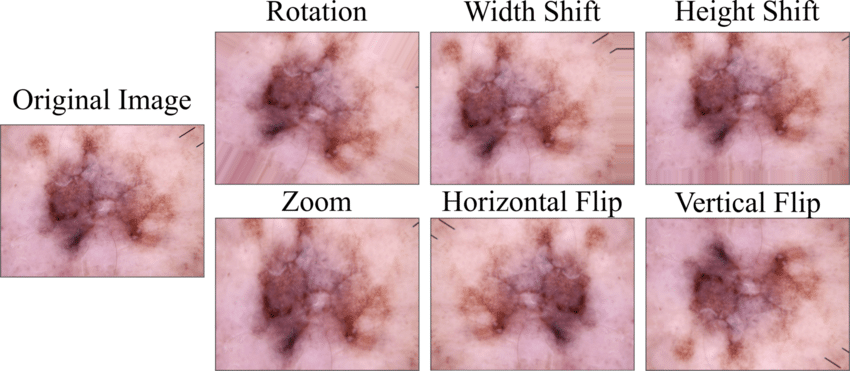
\includegraphics[width=0.8\textwidth]{Data-augmentation.png}
  \caption{Visualization of the data augmentation pipeline applied to a sample image. This figure would illustrate the sequence of transformations such as resizing, random cropping, flips, and color jittering.}
  \label{fig:data-augmentation-pipeline}
\end{figure}

\begin{itemize}
\item \textbf{Resize:} scale images to \texttt{(450, 600)} (height, width)
\item \textbf{RandomResizedCrop:} size=(450, 600), scale=(0.8--1.0)
\item Horizontal and vertical flips ($p=0.5$)
\item Brightness and contrast perturbations ($p=0.3$)
\item Pixel normalization to zero mean and unit variance
\end{itemize}
A custom \texttt{ClassificationDataset} loads images and labels, while a \texttt{WeightedRandomSampler} biases sampling toward under-represented classes.

% Showcase the two MoE model variants separately
\subsubsection*{Small  Model}
This lightweight configuration prioritizes computational efficiency and rapid inference for resource-constrained environments. The architecture employs:
\begin{itemize}
  \item \textbf{Specialist Experts:} EfficientNet-B2, EfficientNet-B3, and EfficientNet-B4 (TIMM implementations: \texttt{efficientnet\_b2}, \texttt{efficientnet\_b3}, \texttt{efficientnet\_b4})
  \item \textbf{Generalist Expert:} EfficientNet-B5 (\texttt{efficientnet\_b5})
\end{itemize}
This configuration balances model complexity with deployment feasibility, making it suitable for edge computing applications and real-time diagnostic scenarios.

\subsubsection*{Large  Model}
This high-capacity configuration maximizes classification accuracy through state-of-the-art deep learning architectures. The ensemble comprises:
\begin{itemize}
  \item \textbf{Specialist Experts:} ConvNeXt Base (\texttt{convnext\_base\_in22ft1k}), EfficientNetv2 Large (\texttt{tf\_efficientnetv2\_l}), and MobileNetV3 Large (\texttt{mobilenetv3\_large\_100})
  \item \textbf{Generalist Expert:} ConvNeXt Base (\texttt{convnext\_base\_in22ft1k})
\end{itemize}
This configuration leverages advanced convolutional architectures and transformer-inspired designs to achieve superior performance on complex dermatological classification tasks, albeit with increased computational requirements.

Our Mixture-of-Experts (MoE) framework integrates specialist and generalist feature extractors:

\begin{figure}[H]
  \centering
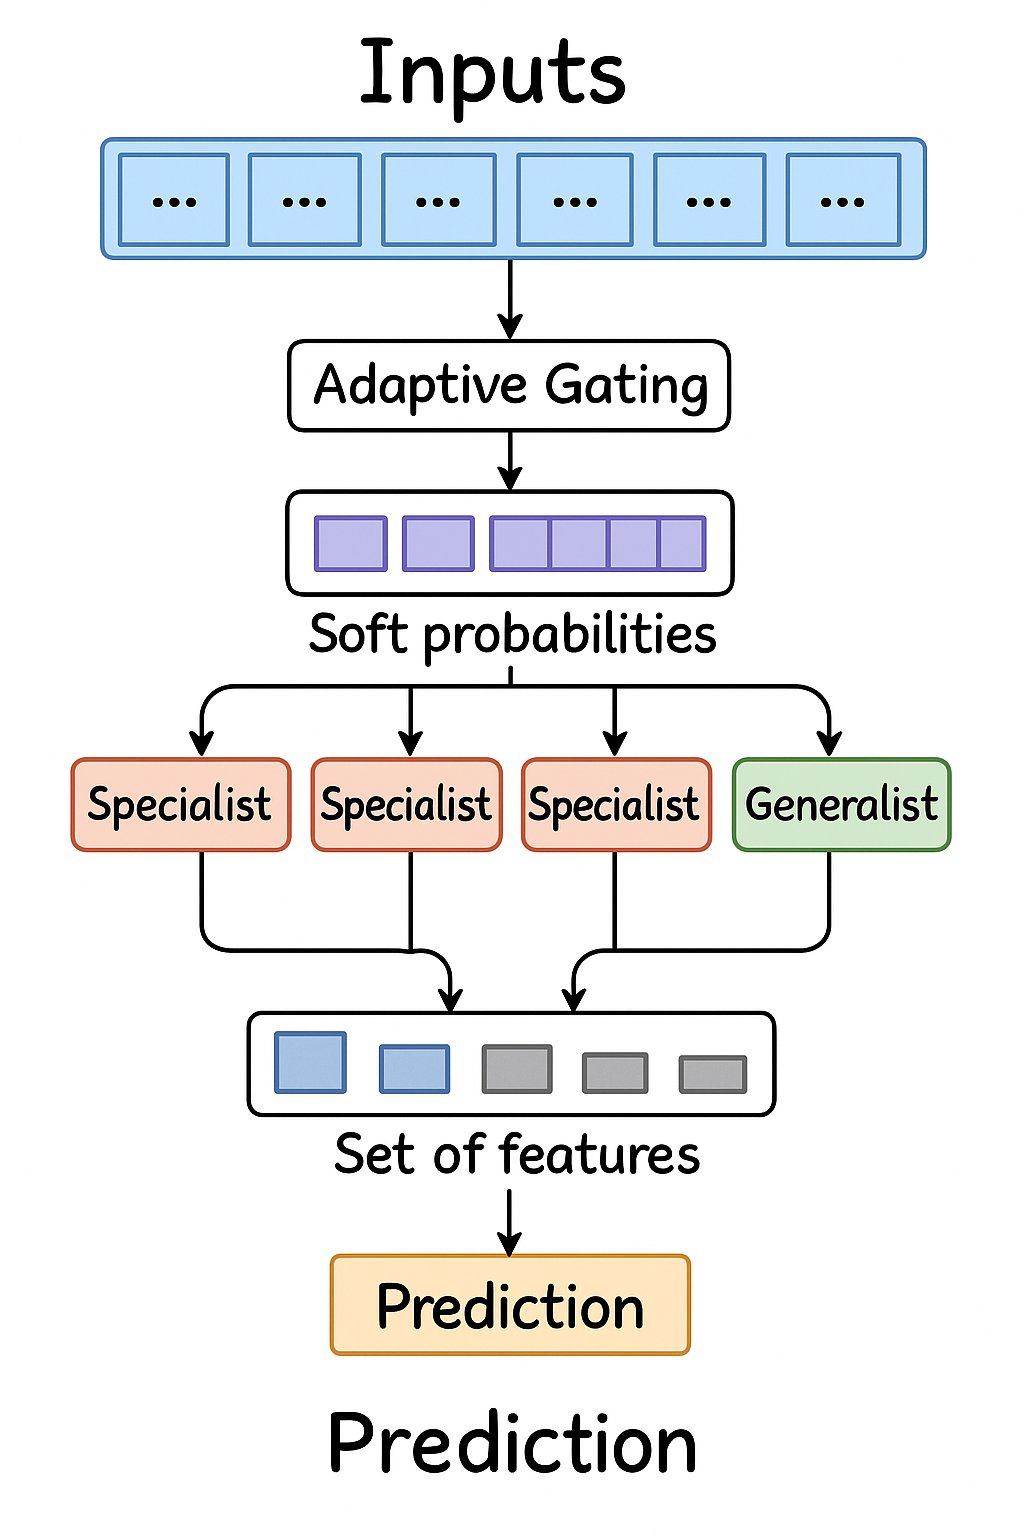
\includegraphics[width=0.6\textwidth]{model_archicture.png}
  
  \caption{High-level architecture of the Mixture-of-Experts (MoE) model. This diagram would show the specialist experts , and the gating network that dynamically weights their contributions.}
  \label{fig:model-architecture}
\end{figure}



\paragraph{Enforcing Specialist Specialization}
To ensure each EfficientNet specialist focuses on distinct data distributions, we employ three complementary mechanisms:
\begin{enumerate}
\item \textbf{Top-$k$ Selection:} At each forward pass, we compute gating scores $g_i$ for all experts using softmax normalization. The softmax converts the raw gating outputs into confidence percentages, indicating how confident the model is in each expert's prediction. The top two experts with the highest confidence scores are then selected:
\begin{equation*}
  \{i_1, i_2\} = \underset{i}{\text{arg top-2}}\, g_i. \cite{shazeer2017outrageously}
\end{equation*}
Only these top two experts contribute to the final prediction by combining their outputs with the corresponding gating weights. This mechanism ensures that the final decision leverages the experts most confident in handling the given input, thus enhancing performance and robustness.

\item \textbf{Load-Balancing Penalty:} We add a regularization term
  \begin{equation*}
    \mathcal{L}_{\text{load}} = \sum_{i=1}^{N_{\text{spec}}} \Bigl(\bar{g}_i - \tfrac{1}{N_{\text{spec}}}\Bigr)^2. \cite{shazeer2017loadbalancing}
  \end{equation*}
 where for each specialist $i$,
  \begin{align*}
    g_{b,i} &= \text{softmax\_weight}_{b,i}  \quad\text{(gate weight for sample $b$)},\\
    \bar{g}_i &= \frac{1}{B} \sum_{b=1}^{B} g_{b,i}  \quad\text{(batch-average weight)},
  \end{align*}
  and $B$ is the batch size. This penalty is added to the overall loss, so during backpropagation the gating network's parameters are updated not only to improve classification but also to push each $\bar{g}_i$ toward the uniform target $1/N_{\text{spec}}$. In practice, gradients of $\mathcal{L}_{\text{load}}$ flow through the softmax gate, encouraging under-utilized experts to change weights and over-utilized ones , that are becoming more like a generalist , to do the same ,by doing so we force both types of experts  to specialize.
\item \textbf{Generalist Bias Floor:} We add a fixed bias ($0.4$) to the generalist’s score before softmax, ensuring a minimum participation floor that prevents specialists from being completely overshadowed and maintaining a balanced expert ensemble.
\end{enumerate}
These mechanisms collectively drive each EfficientNet-b2/b3/b4 expert to specialize on subsets of the skin lesion data, while the generalist provides robust fallback coverage.

\section{Training Protocol}
Training uses mixed precision (AMP) with the AdamW optimizer (lr=$1\times10^{-4}$, weight decay=$1\times10^{-4}$). The combined loss is:
\begin{equation}
\mathcal{L} = \mathcal{L}_{\mathrm{CE}} + \lambda_{bal} \cdot \mathcal{L}_{\mathrm{load}}. \cite{shazeer2017loadbalancing}
\end{equation}
where $\mathcal{L}_{\mathrm{CE}}$ is cross-entropy and $\mathcal{L}_{\mathrm{load}}$ penalizes uneven expert utilization. Here, $\lambda_{bal}$ is a hyperparameter that controls the trade-off between the classification loss and the load balancing regularization term. We train for up to 40 epochs with a batch size of 16 and implement early stopping after 5 epochs without improvement. A \texttt{ReduceLROnPlateau} scheduler halves the learning rate when balanced accuracy plateaus. All random seeds are fixed for reproducibility.

\section{Evaluation}
At each epoch, we evaluate on a held‑out validation set, logging per‑class precision, recall, and F1‑score via \texttt{sklearn.metrics.classification\_report}, and report balanced accuracy to mitigate class imbalance. Final evaluation runs on a reserved test split.

\subsection*{Evaluation Metrics}
To comprehensively assess the performance of our model, we employ a suite of standard evaluation metrics [5,6]. Each metric provides a different perspective on the model's classification capabilities:

\begin{itemize}
    \item \textbf{Accuracy:} This metric represents the proportion of all predictions that were correct. It is calculated as:
    \begin{equation}
        \text{Accuracy} = \frac{\text{Number of Correct Predictions}}{\text{Total Number of Predictions}}
    \end{equation}

    \item \textbf{Precision:} For a given class, precision measures the proportion of positive identifications that were actually correct, i.e., $\frac{\mathrm{TP}}{\mathrm{TP}+\mathrm{FP}}$.

    \item \textbf{Recall (Sensitivity):} The proportion of actual positives correctly identified: $\frac{\mathrm{TP}}{\mathrm{TP}+\mathrm{FN}}$.

    \item \textbf{F1-Score:} The harmonic mean of precision and recall: $2\frac{\mathrm{Precision}\cdot\mathrm{Recall}}{\mathrm{Precision}+\mathrm{Recall}}$.

    \item \textbf{Balanced Accuracy:} The mean of recall across all classes: $\frac{1}{C}\sum_{i=1}^{C}\mathrm{Recall}_i$.
    As defined in \cite{litjens2017survey}

    \item \textbf{Macro Average:} For metrics like precision, recall, and F1-score, the macro average is calculated by taking the arithmetic mean of the metric for each class, without considering class imbalance. Each class contributes equally to the average.

    \item \textbf{Weighted Average:} Similar to the macro average, but each class's metric is weighted by its support (the number of true instances for that class). This average is more influenced by the performance on larger classes.

\end{itemize}

These metrics, reported per-class and as macro/weighted averages, allow a nuanced understanding of model performance.



\section{Conclusion}
This chapter detailed our end‑to‑end methodology for skin lesion classification, from balanced data augmentation through a Mixture‑of‑Experts model, rigorous training, and evaluation, to plans for edge deployment. We demonstrated feasible training on consumer‑grade hardware (RTX 3060 Lite, 12 GB VRAM; 32 GB RAM; Ryzen 7 CPU) and outlined future directions for TPU‑accelerated inference.

% Add equation sources section
\section*{Equation Sources and References}
\begin{enumerate}
  \item \textbf{Top-\(k\) Expert Selection}\\
    Equation:
    \begin{equation*}
      \{i_1, i_2\} = \mathrm{arg\,top\text-2}_i\,g_i
    \end{equation*}
    Source: \cite{shazeer2017outrageously}
  
  \item \textbf{Load-Balancing Penalty}\\
    Equation:
    \begin{equation*}
      \mathcal{L}_{\text{load}} = \sum_{i=1}^{N_{\text{spec}}} \bigl(\bar{g}_i - \tfrac{1}{N_{\text{spec}}}\bigr)^2
    \end{equation*}
    Source: \cite{shazeer2017loadbalancing}
  
  \item \textbf{Generalist Bias Floor}\\
    Concept: Add a fixed bias to the generalist’s gating score before softmax to ensure minimum participation.
    Source: \cite{shazeer2017outrageously}
\end{enumerate}

%%% Local Variables:
%%% mode: latex
%%% TeX-master: "isae-report-template"
%%% End:
